\documentclass{report}
\usepackage{tikz}
\usepackage{subcaption}

\begin{document}
\begin{figure}
  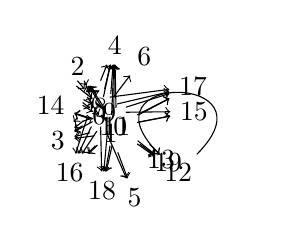
\begin{tikzpicture}
      \draw
        (-0.255, 0.112) node (0){0}
        (-0.109, -0.115) node (1){1}
        (-0.335, 0.32) node (7){7}
        (-0.244, 0.211) node (8){8}
        (-0.531, 0.73) node (2){2}
        (-0.129, 0.154) node (9){9}
        (-0.075, -0.031) node (10){10}
        (-0.038, -0.024) node (11){11}
        (-0.783, -0.205) node (3){3}
        (-0.06, 1.0) node (4){4}
        (0.192, -0.922) node (5){5}
        (0.746, -0.615) node (12){12}
        (0.529, -0.442) node (13){13}
        (-0.872, 0.242) node (14){14}
        (0.316, 0.861) node (6){6}
        (0.946, 0.166) node (15){15}
        (-0.632, -0.608) node (16){16}
        (0.935, 0.487) node (17){17}
        (-0.22, -0.834) node (18){18}
        (0.62, -0.488) node (19){19};
      \begin{scope}[->]
        \draw (0) to (1);
        \draw (0) to (2);
        \draw (0) to (9);
        \draw (0) to (10);
        \draw (0) to (11);
        \draw (0) to (3);
        \draw (0) to (4);
        \draw (0) to (5);
        \draw (0) to (6);
        \draw (1) to (7);
        \draw (1) to (3);
        \draw (1) to (4);
        \draw (1) to (5);
        \draw (7) to (8);
        \draw (7) to (2);
        \draw (7) to (9);
        \draw (7) to (3);
        \draw (7) to (4);
        \draw (7) to (16);
        \draw (7) to (17);
        \draw (8) to (2);
        \draw (8) to (9);
        \draw (8) to (3);
        \draw (8) to (4);
        \draw (8) to (16);
        \draw (8) to (17);
        \draw (8) to (18);
        \draw (9) to (2);
        \draw (9) to (3);
        \draw (9) to (4);
        \draw (9) to (15);
        \draw (9) to (16);
        \draw (9) to (17);
        \draw (9) to (18);
        \draw (10) to (2);
        \draw (10) to (3);
        \draw (10) to (4);
        \draw (10) to (12);
        \draw (10) to (14);
        \draw (10) to (15);
        \draw (10) to (16);
        \draw (10) to (17);
        \draw (10) to (18);
        \draw (11) to (2);
        \draw (11) to (4);
        \draw (11) to (12);
        \draw (11) to (14);
        \draw (11) to (15);
        \draw (11) to (16);
        \draw (11) to (17);
        \draw (11) to (18);
        \draw[loop,] (12) to (12);
        \draw (13) to (12);
        \draw (19) to (12);
      \end{scope}
    \end{tikzpicture}
  \caption{Structure of test.tex}\label{fig1}
\end{figure}
\end{document}